\section{Результаты вычислительного эксперимента}
%
%
%
%
\par
Примененные численные методы демонстрировали сходимость к оптимальному решению балки, с определением формы балки и частоты безрезонансных колебаний балки, с учетом заданных параметров проектирования (толщины, массы), при ограничении на толщину.
%
%
%
\begin{enumerate}
	\item 	$h(x) = 2\sqrt{x}$; \;\; $u_{min} = 0{,}4$; \;\; $u_{max} = 1{,}8$
	\item 	$h(x) = 181.263 \rho^2e/x^6 $; \;\; $u_{min} = 0{,}4$; \;\; $u_{max} = 1{,}8$
\end{enumerate}

\begin{center}
	\begin{figure}
		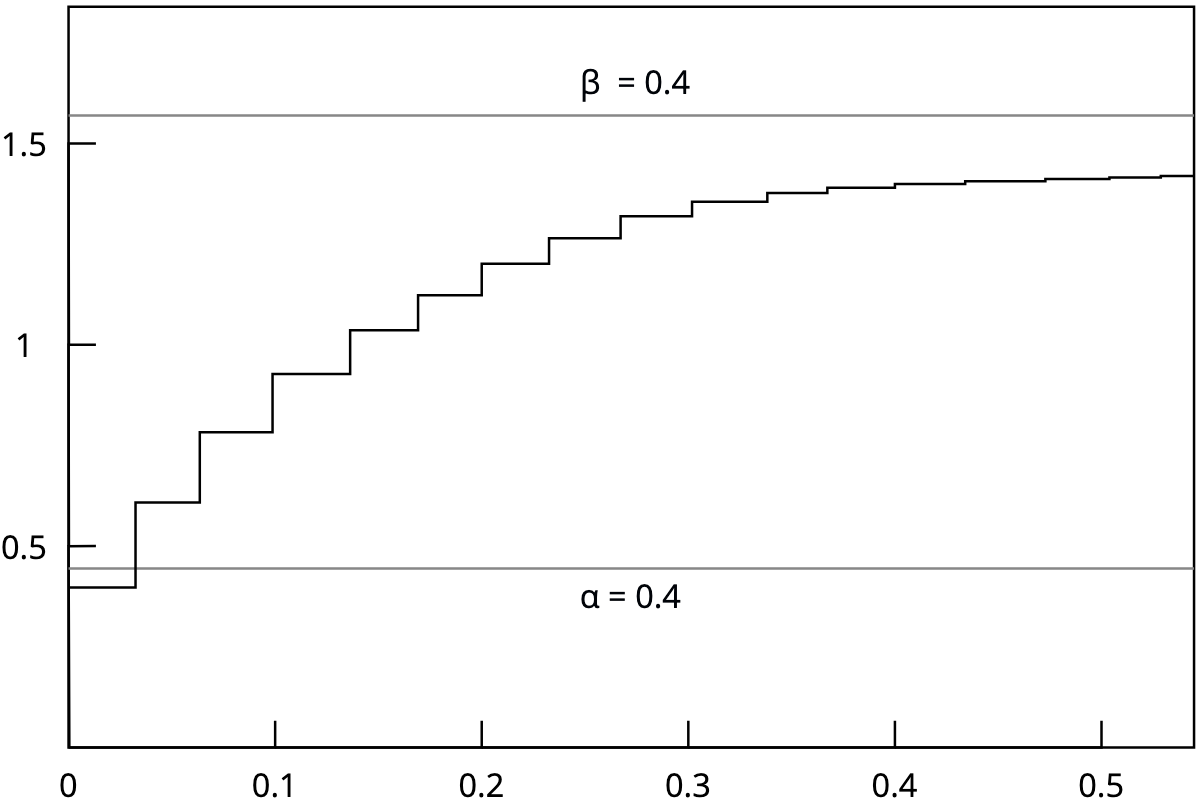
\includegraphics[width=1\linewidth]{untitled2.png}
		\caption{Оптимальное распределение толщины балки $u_{opt}$ (1).}
		\bigskip
		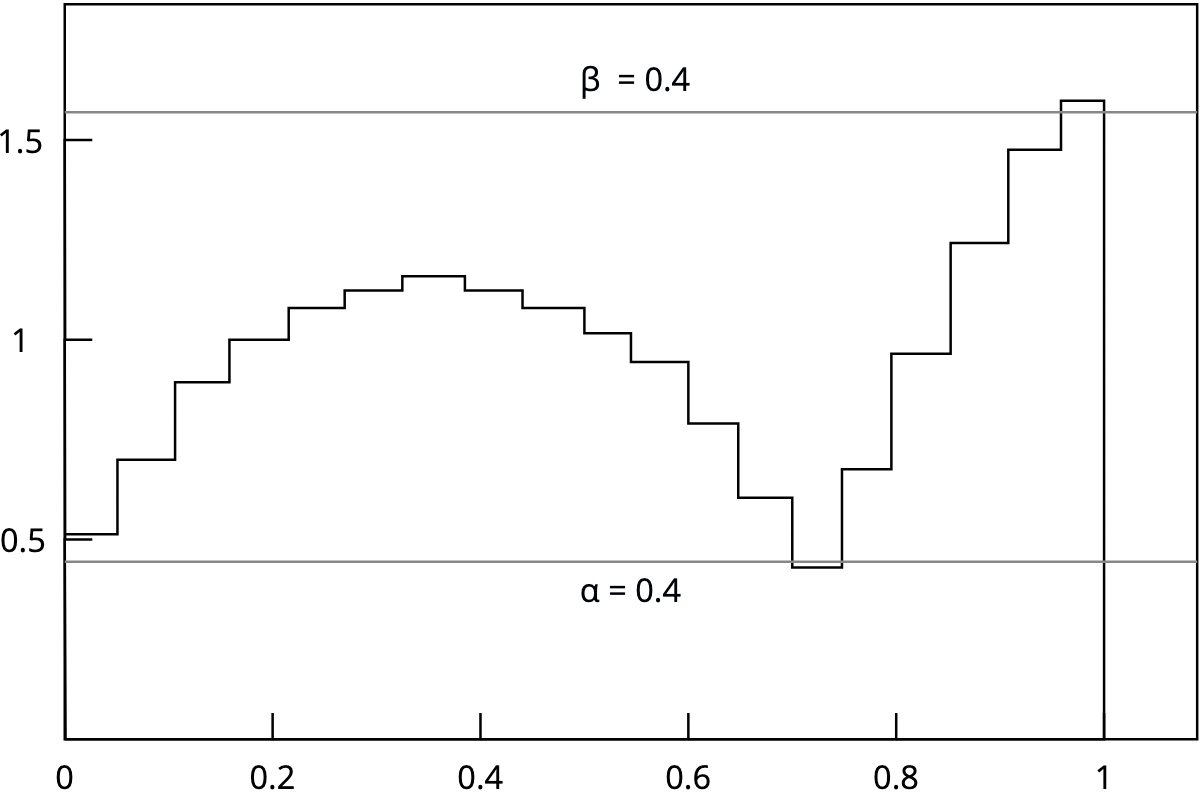
\includegraphics[width=1\linewidth]{untitled.png}
		\caption{Оптимальное распределение толщины балки $u_{opt}$ (2).}
	\end{figure}
	%
	%
	%
\end{center}



%Картинки.

%При каких параметрах получены.

%Каков эффект оптимизации.

%Анализ.

%Параметры $\alpha, \beta, \nu$.

%Оптимальное распределение
%Оптимизация эффективность




%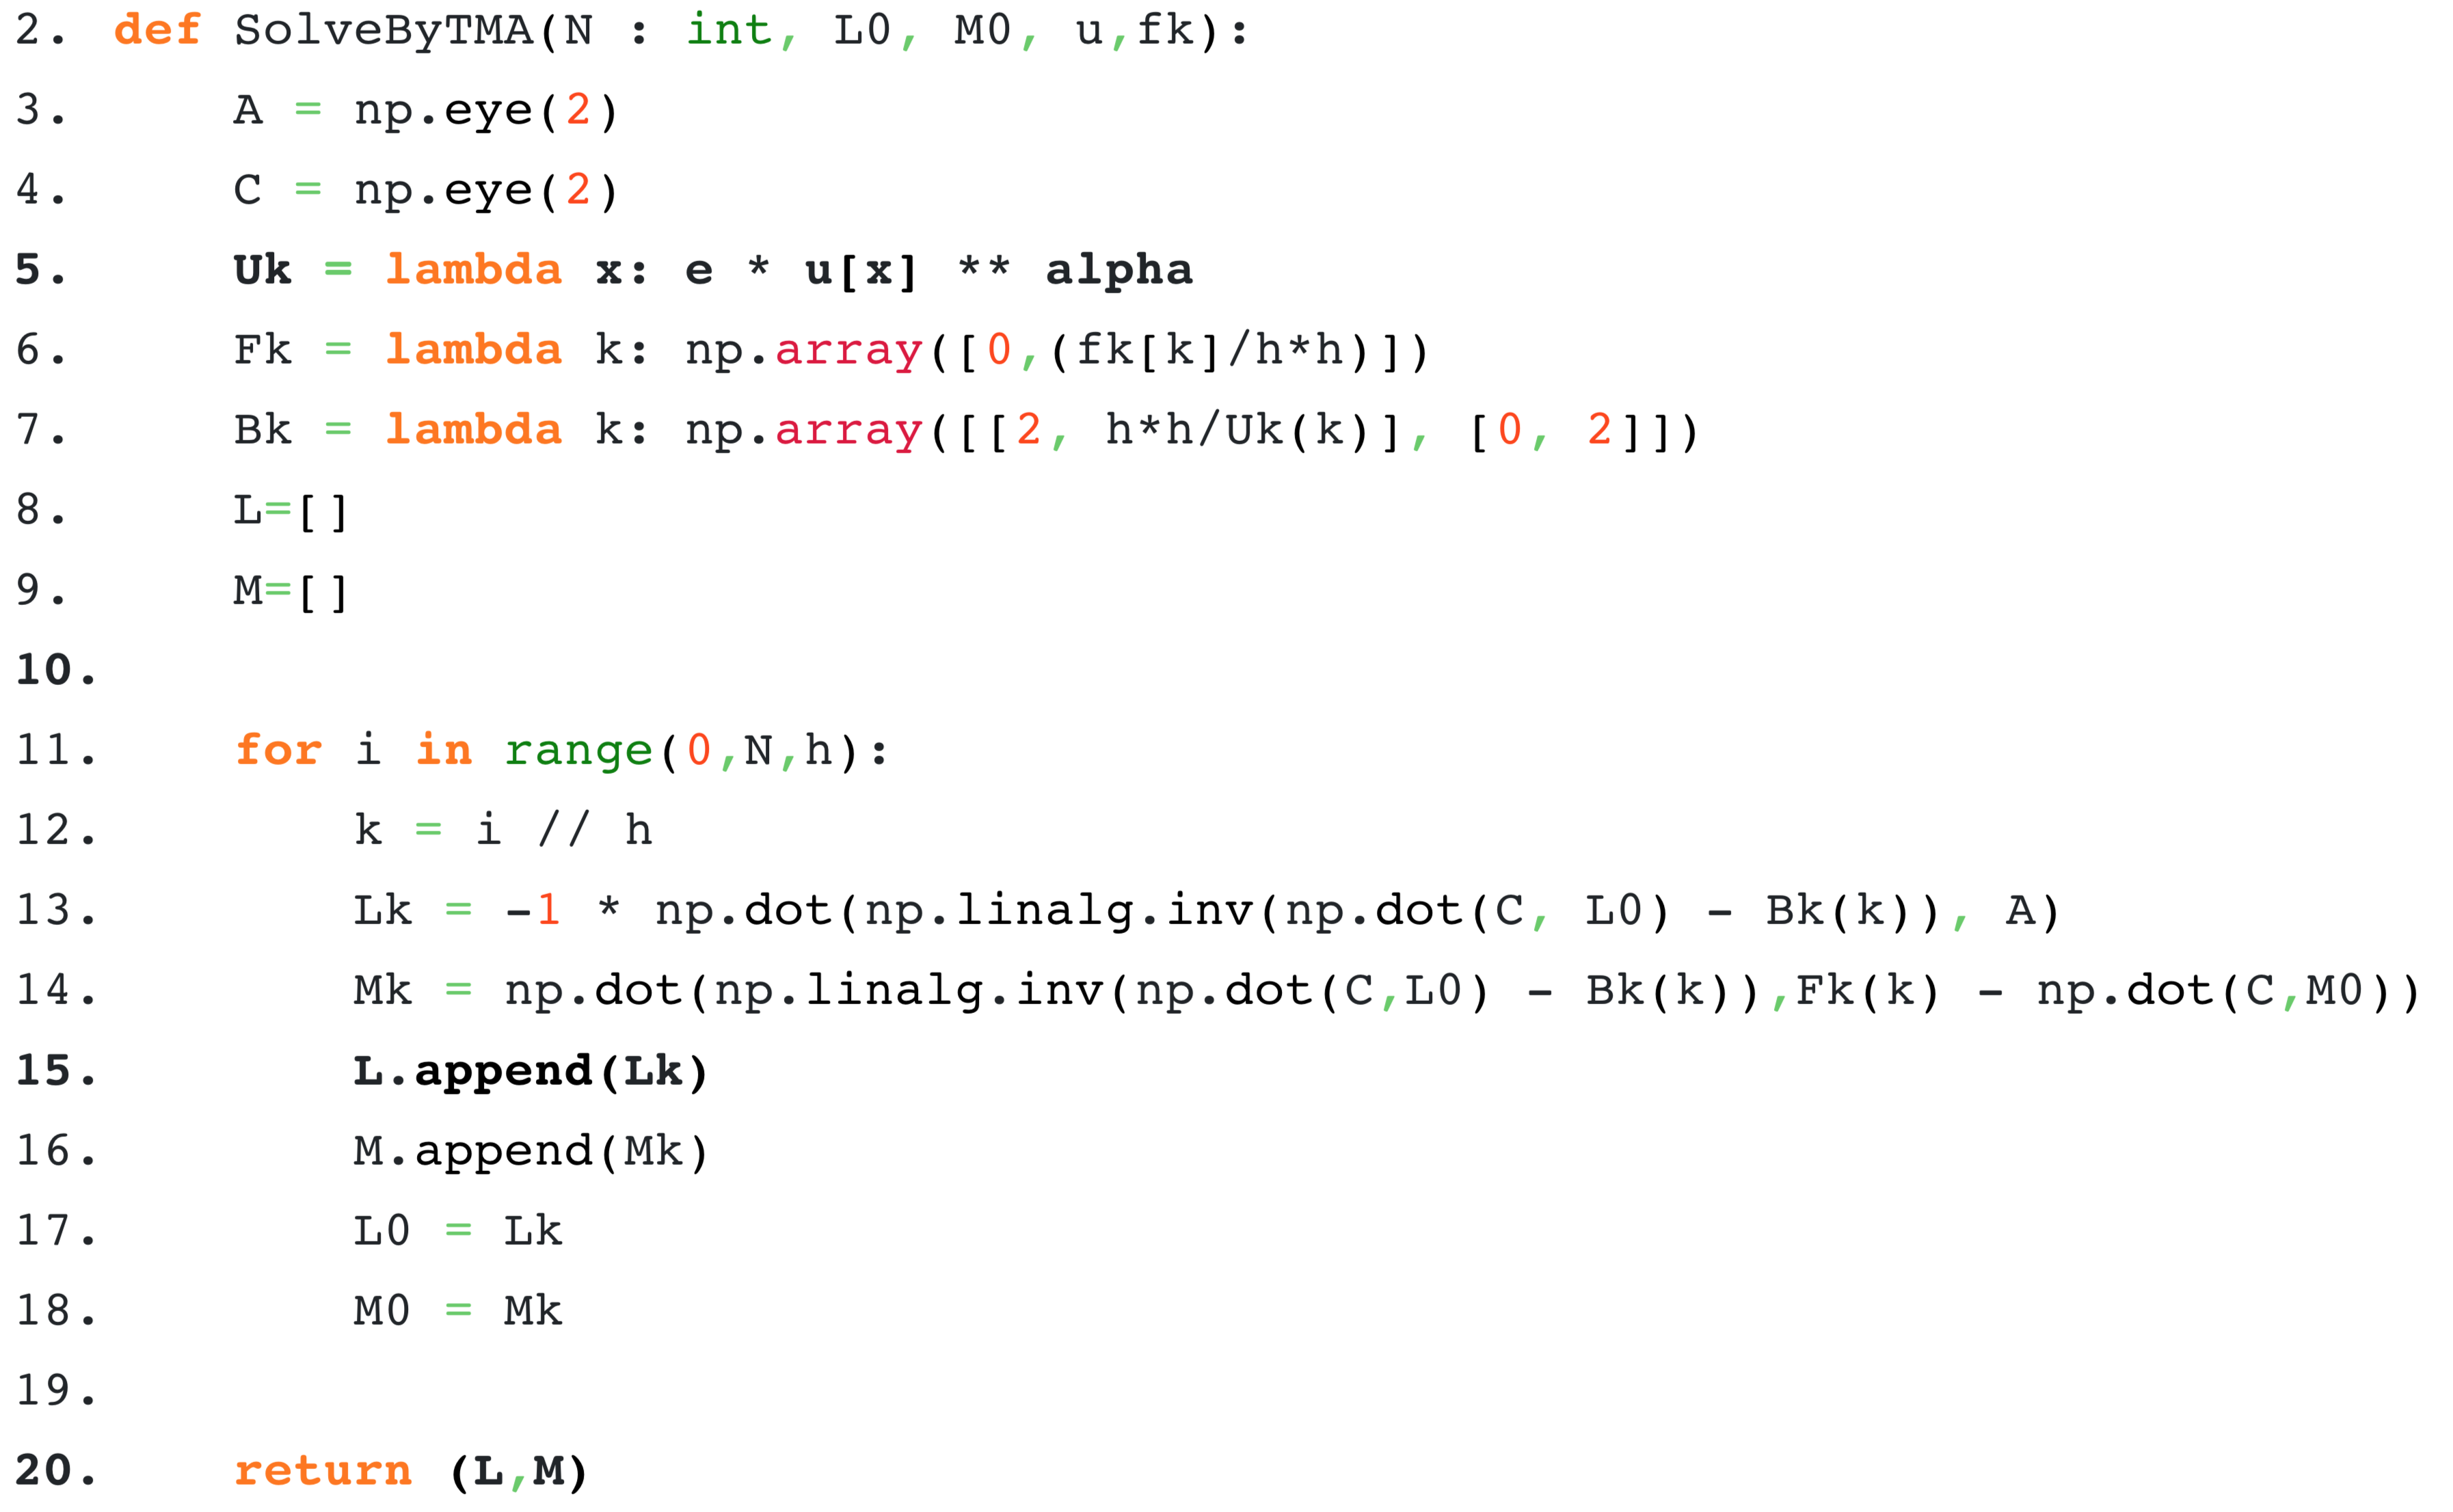
\includegraphics[width=0.5\linewidth]{1code.png}
%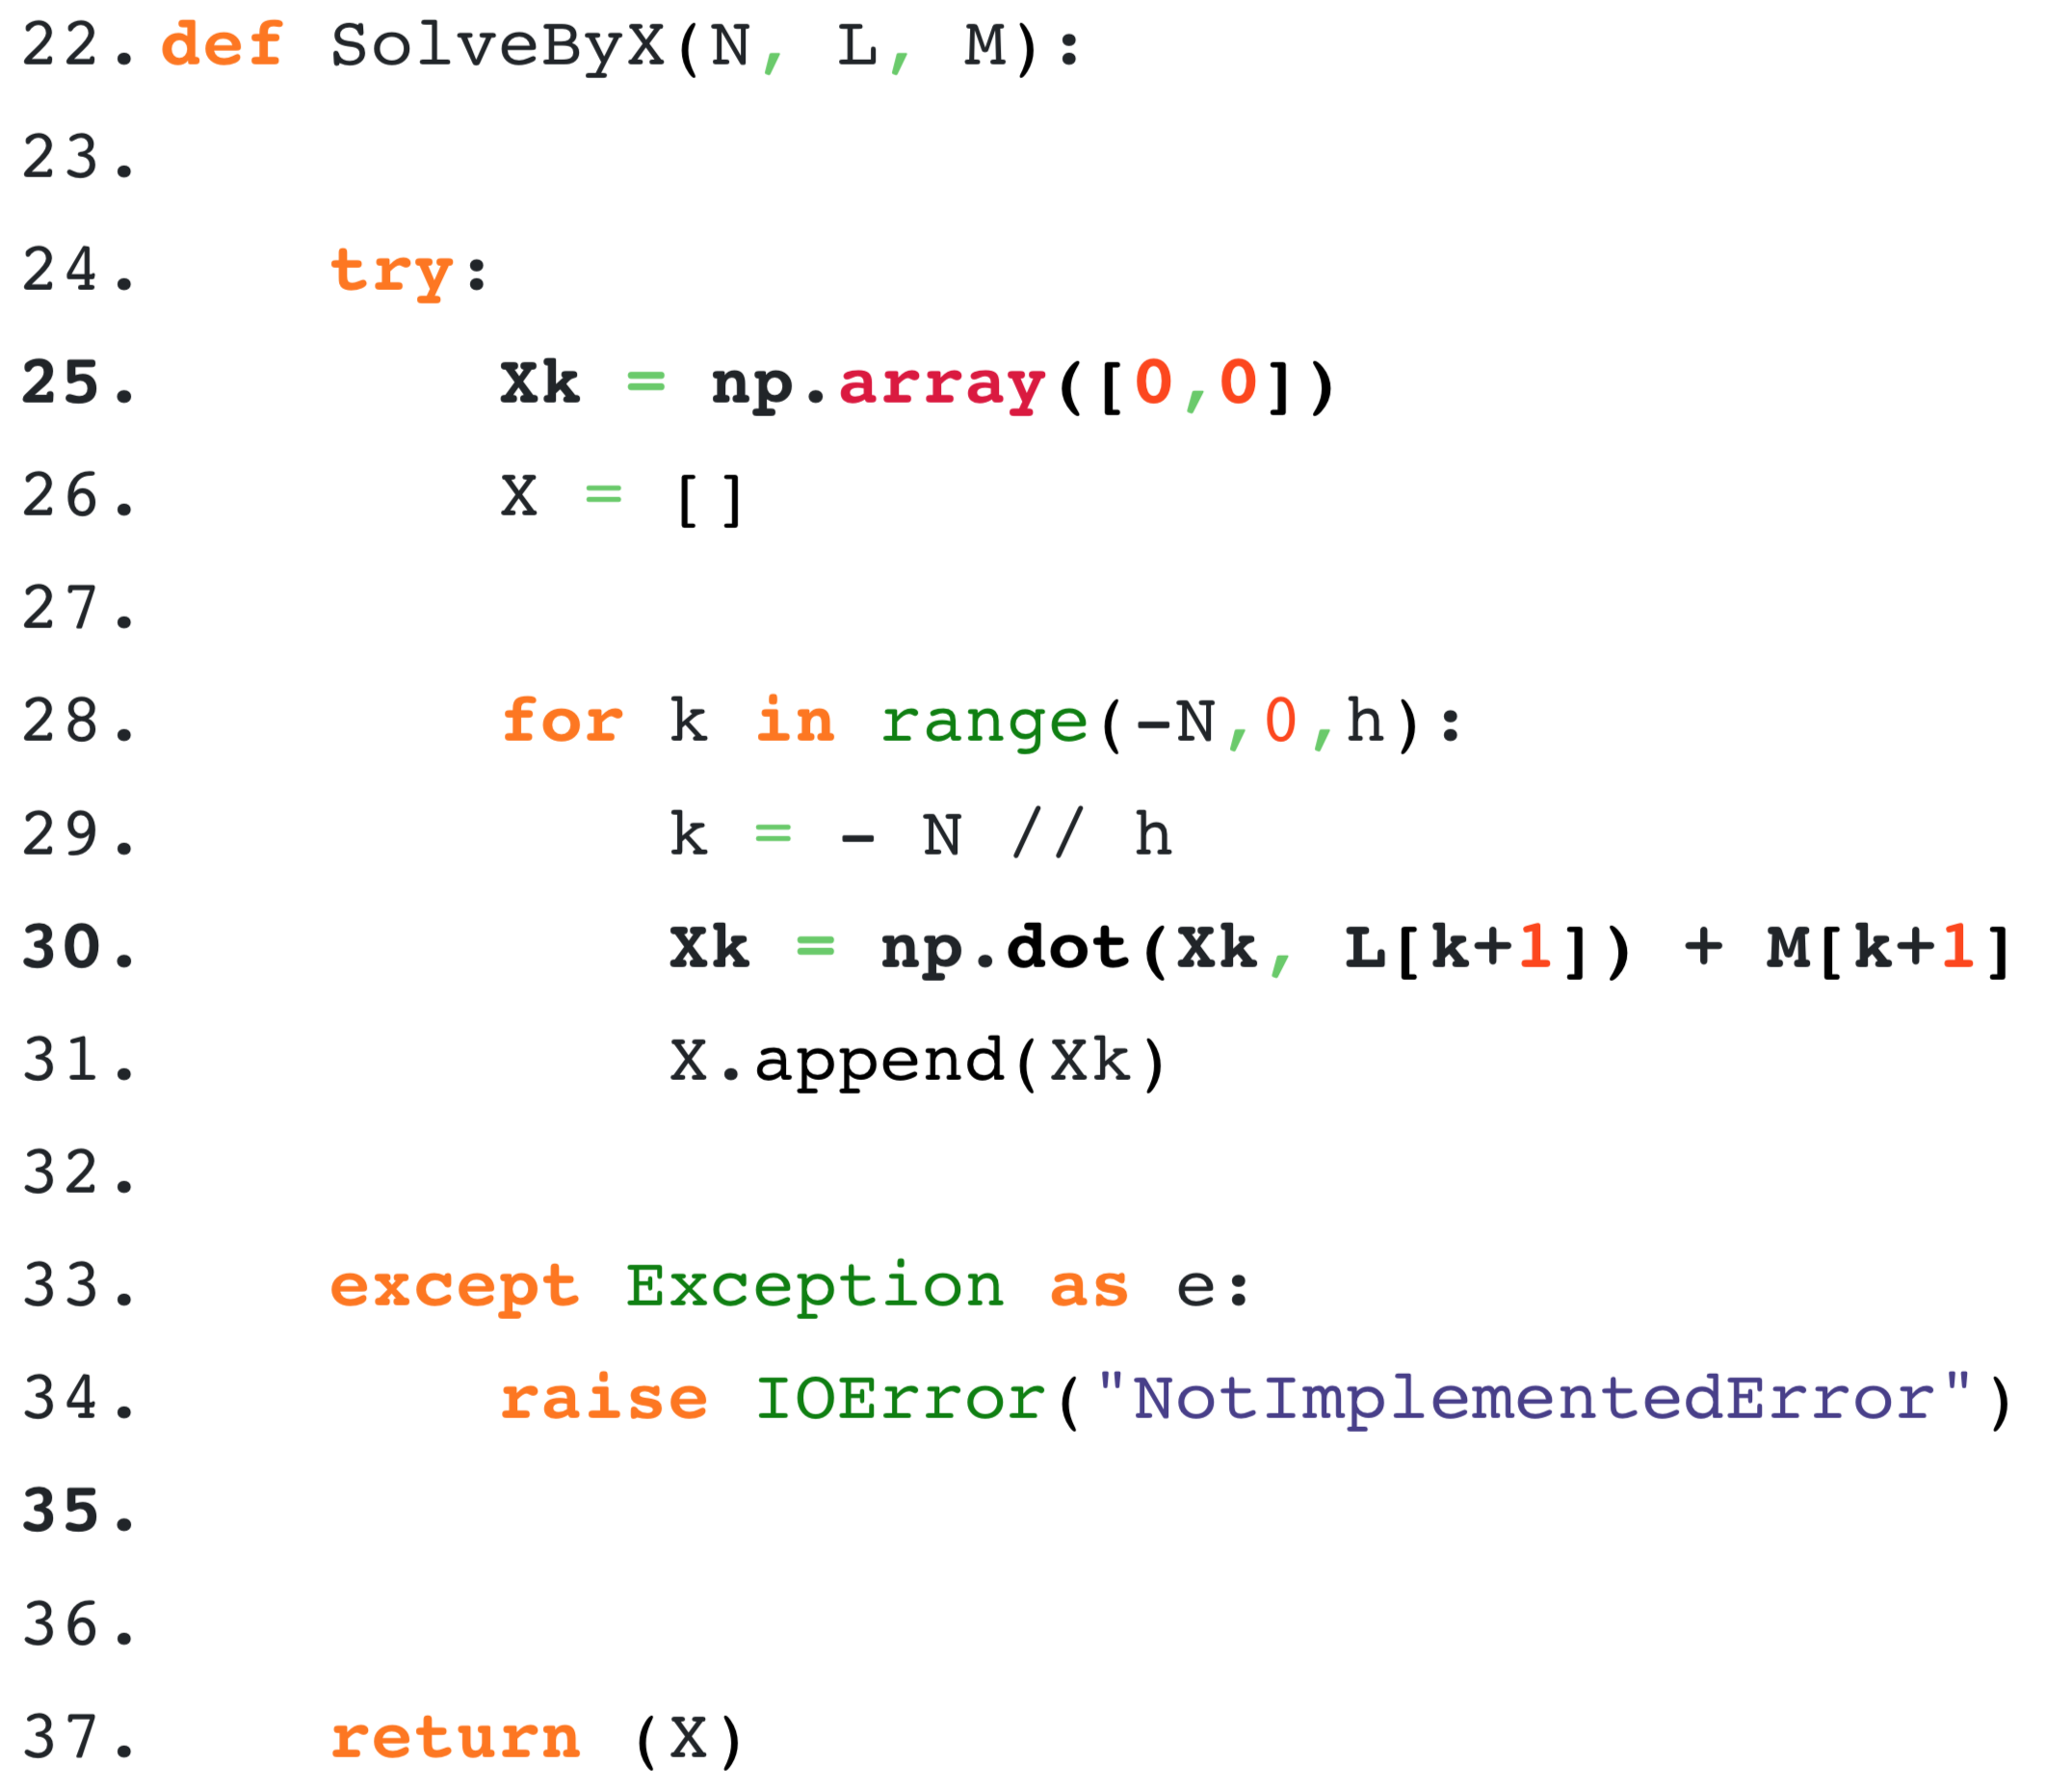
\includegraphics[width=0.5\linewidth]{2code.png}
%\\
%При каких параметрах получены.
%
%Каков эффект оптимизации.
%
%Анализ.
%
%Параметры $\alpha, \beta, \nu$.